\documentclass[11pt]{article}

\usepackage[margin=1in]{geometry}
\usepackage{amsmath, amssymb, amsthm}
\usepackage{bm}
\usepackage{booktabs}
\usepackage{graphicx}
\usepackage{longtable}
\usepackage{enumitem}
\usepackage{hyperref}
\usepackage{xcolor}
\usepackage{listings}
\usepackage{verbatim}

\hypersetup{
  colorlinks=true,
  linkcolor=blue!50!black,
  urlcolor=blue!50!black,
  citecolor=blue!50!black
}

\lstset{
  basicstyle=\ttfamily\footnotesize,
  breaklines=true,
  showstringspaces=false,
  frame=single,
  framesep=4pt,
  keywordstyle=\color{blue!60!black}\bfseries,
  commentstyle=\color{gray!70!black}\itshape,
  stringstyle=\color{red!60!black},
  language=Python
}

\newcommand{\code}[1]{\texttt{#1}}
\newcommand{\file}[1]{\texttt{\small #1}}
\newcommand{\pgen}{p_{\text{gen}}}
\newcommand{\pswap}{p_{\text{swap}}}
\newcommand{\pfusion}{p_{\text{fusion}}}

\title{Qamel / Timing-Multiuser-Protocols:\\
A Complete Codebase Reference for Collaborating Models}
\author{Internal technical memo\\(generated for the Claude $\leftrightarrow$ Claude Code collaboration loop)}
\date{June 19, 2026}

\begin{document}
\maketitle

\begin{abstract}
This document is a self-contained reference to the \code{Timing-Multiuser-Protocols} repository (project codename \emph{Qamel}). It is written so that another model with a stronger grasp of the physics --- entanglement distribution in quantum repeater chains, multipartite generation with fusion, and the latency budget of quantum SDN --- can read it once and then meaningfully collaborate on the existing reinforcement learning (RL) implementation. The document does \emph{not} re-derive any code beyond what is necessary to understand the design choices and pitfalls. Where the code disagrees with the README or with the paper's framing, that disagreement is flagged explicitly. The aim is to maximize agent--agent collaboration efficiency: after reading this, the second Claude should be able to suggest physics-aware modifications without further code spelunking.
\end{abstract}

\tableofcontents
\clearpage

\section{Latest Implementation and Result Log (through June 19, 2026)}
\label{sec:latest-log}

This log records the current state of the reinforcement-learning branch after the June 11, 2026 integration pass.

\begin{itemize}
  \item Added an optional dueling DQN architecture, selected with \code{--dueling}. The original \code{DQNNet} remains the default. The dueling trunk now uses the same \code{net.1} and \code{net.3} state-dict keys as the original network trunk, so trunk weights can be copied from a plain DQN checkpoint into a dueling model by matching keys. A bug was found during this audit where the dueling trunk was named \code{trunk.*}; that made the checkpoint keys disjoint from \code{DQNNet}. This was fixed on June 11, 2026.
  \item Added optional Double DQN updates with \code{--double-dqn}. When enabled, the policy net selects the next valid action and the target net evaluates it.
  \item Added optional potential-based reward shaping with \code{--pbrs} and \code{--pbrs-scale}. The potential is $\Phi(s)$, the length of the longest contiguous run of elementary links starting at node 0. Training stores the shaped reward in replay but still logs the unshaped environment reward.
  \item Split replay-buffer terminal flags into \code{terminated} and \code{truncated}; truncated transitions now continue to bootstrap in the Bellman target. Legacy five-field replay entries are still loadable, but their old \code{done} flag cannot distinguish true termination from timeout.
  \item Added \file{scripts/head\_to\_head.py}, a seeded comparison harness for \code{dqn\_greedy}, \code{dqn\_swapprefer}, and a non-neural heuristic. It reads \file{config.json}, prefers \file{checkpoints/best\_eval.pt}, writes JSON with per-seed summaries, and prints a Markdown table.
  \item Updated evaluation model construction to use the checkpoint/config architecture selector, so \code{evaluate\_qamel.py} can load either plain or dueling DQN checkpoints.
  \item Current syntax/import checks pass for \code{qamel.dqn}, \code{qamel.utils}, \code{scripts.train\_qamel}, \code{scripts.evaluate\_qamel}, and \code{scripts.head\_to\_head}. No long training run was executed as part of this log.
\end{itemize}

\subsection{Lab notebook entry: Myriad status on June 17, 2026}
\label{sec:lablog-2026-06-17}

The cluster status check on UCL Myriad found no active queued/running jobs from
\code{qstat -u "\$USER"}. The submitted artifacts are therefore either completed,
failed, or terminated by the scheduler. The relevant evidence came from
\file{qamel/outputs/studies/*/cross\_budget\_summary.csv},
\file{qamel/outputs/cluster\_logs/*.out}, and
\file{qamel/outputs/stage0\_escalation\_logs/*.out}.

\begin{center}
\begin{tabular}{llrrl}
\toprule
Run tag & Source & Budget & Success rate & Status \\
\midrule
\code{lq\_n5\_seed12345\_progressive} & Myriad archive & 1{,}000 & 0.024 & archived \\
\code{lq\_n5\_seed12345\_progressive} & Myriad archive & 5{,}000 & 0.506 & archived \\
\code{lq\_n5\_seed12345\_progressive} & Myriad archive & 10{,}000 & 0.904 & archived \\
\code{lq\_n5\_seed12345\_progressive} & checkpoint dir & 11{,}000 & -- & checkpoint exists, no eval archive \\
\code{lq\_n6\_seed12345\_progressive} & Myriad archive & 1{,}000 & 0.162 & archived \\
\code{lq\_n6\_seed12345\_progressive} & Myriad archive & 2{,}000 & 0.012 & archived \\
\code{lq\_n6\_seed12345\_progressive} & Myriad archive & 3{,}000 & 0.208 & archived \\
\code{lq\_n6\_seed12345\_progressive} & Myriad archive & 4{,}000 & 0.000 & archived \\
\code{swapaware\_seed12345} & Myriad archive & 200 & 0.204 & archived, later resume failed \\
\bottomrule
\end{tabular}
\end{center}

Interpretation:
\begin{itemize}
  \item The strongest confirmed cluster result remains the single-seed $n=5$,
  $\pgen=0.4$, $\pswap=0.7$ progressive run at 10{,}000 training episodes:
  success rate $0.904$, mean return $58.618$, mean steps $23.182$, and
  truncated fraction $0.096$ over a 500-episode greedy evaluation.
  \item The planned 20{,}000-episode continuation for that same $n=5$ run did
  start and wrote \file{episode\_011000.pt}, but no
  \file{budget\_20000/eval\_summary.json} was archived. The current lab-book
  state is therefore ``10{,}000 complete; 20{,}000 incomplete'', not ``20{,}000
  failed scientifically''.
  \item The submitted Stage-0 escalation array
  \file{qamel/outputs/stage0\_escalation\_logs/qamel\_s0\_esc.612520.*.out}
  did not train. Every task exited at argument parsing with
  \code{unrecognized arguments: --max\_actions 100 --double-dqn --dueling --pbrs
  --pbrs-scale 1.0 --lr 5e-4 --batch\_size 256}. This is an operational
  failure: the Myriad checkout was stale and did not contain the newer training
  CLI flags.
  \item Later $n=6$ progressive submissions attempted to resume an old
  checkpoint whose hidden width was 512, while the current $n=6$ model width is
  768 under the formula in \S\ref{sec:rl}. The resulting
  \code{size mismatch} is expected; $n=6$ must be restarted under a fresh run tag
  or after moving the legacy checkpoint directory aside.
  \item The \code{swapaware\_seed12345} run archived a 200-episode evaluation but
  then failed on resume because the stale cluster code tried to restore an RNG
  state that was not a \code{torch.ByteTensor}. The current local training code
  converts restored RNG tensors before calling \code{torch.random.set\_rng\_state},
  but this must be confirmed on Myriad after a clean \code{git pull}.
\end{itemize}

Immediate operational conclusion: before any new Stage-0, dueling, Double-DQN,
PBRS, or publication-suite job is submitted on Myriad, the cluster checkout must
be made clean enough for \code{git pull --ff-only}. Otherwise the scheduler will
keep running older scripts that reject the new flags.

\subsection{Lab notebook entry: $n=6$ no-go and $n=7$ control status on June 19, 2026}
\label{sec:lablog-2026-06-19-n6-n7}

The running Myriad arrays were inspected using both the rolling training proxy
and every available greedy best-evaluation check. The greedy trajectories change
the interpretation: the current $n=6$ configuration is unstable rather than
merely slow to learn. It is a \textbf{no-go for a full multi-seed claim}. The
already-running tasks are pilots; held seeds should not be released under this
configuration.

\begin{center}
\small
\begin{tabular}{p{0.08\textwidth}p{0.58\textwidth}p{0.25\textwidth}}
\toprule
Seed & Greedy evaluation trajectory & Interpretation \\
\midrule
202 & $0.03 \rightarrow 0.62$ (6k) $\rightarrow 0.51$ (8k) $\rightarrow 0.25$ (10k)
    & learn then collapse \\
303 & stored peak $0.68$ (4k); $0.025 \rightarrow 0.020 \rightarrow 0.005 \rightarrow 0.015$ (10k--16k)
    & early peak then near-dead \\
404 & $0.08 \rightarrow 0.63$ (4k)
    & healthy so far, still in danger window \\
\bottomrule
\end{tabular}
\end{center}

For seed 202, the rolling training proxy had also fallen to $0.005$ at episode
10{,}400, confirming that the live policy was nearly dead after its 0.62 greedy
peak. The frozen \file{best\_eval.pt} protects the peak artifact from subsequent
degradation. Seed 303 likewise had an early stored 0.68 checkpoint, but its
later greedy checks stayed around 1--2\% with mean steps near 98, indicating
near-constant truncation. This corrects the initial shorthand that seed 303
``never learned'': the complete evidence instead shows a still stronger
learn-then-collapse failure. Seed 404 had reached 0.63 at episode 4{,}000, but
seed 202 was similarly healthy at that age before failing. The current read is
therefore two collapsed seeds and one not-yet-failed seed, versus the clean
$8/8$ $n=5$ Stage-0 result.

\subsubsection*{Working diagnosis}

The dominant configuration problem is the exploration schedule. In
\file{scripts/train\_qamel.py}, \code{eps\_decay\_steps} is measured in
environment steps through \code{steps\_done}, not in episodes. The $n=6$ array
sets it to only 30{,}000 even though the full run is of order 1.3 million or more
environment steps; seed 202 had already accumulated roughly 133k steps by
episode 4{,}000. Epsilon consequently reaches its 0.05 floor by roughly episode
900 and stays there for about 98\% of training. A degraded policy therefore has
almost no exploratory mechanism with which to recover.

The remaining stability settings plausibly amplify this failure at the larger
$n=6$ network/action scale: the array uses a 768-wide network, learning rate
$5\times10^{-4}$, hard target synchronisation every 1{,}000 environment steps,
and gradient clipping at 10.0. The observed early rise followed by a sharp,
persistent drop is consistent with catastrophic forgetting and Q-value
overestimation or moving-target oscillation. This is a working diagnosis, not a
separately instrumented Q-value measurement.

There is also a measurement/configuration bug. The wrappers set the training and
final gate horizon to 150 actions for $n=6$ and 200 for $n=7$, but do not pass
\code{--best\_eval\_max\_actions}; checkpoint selection therefore uses its
default horizon of 100. This explains failing greedy checks with mean steps near
98 and means that ``best'' checkpoint selection is not aligned with the final
head-to-head gate.

The training horizon itself is \emph{not} the indicated lever. Seed 202's 0.62
peak had mean steps 49, showing that the chain is solvable well inside the
existing limit. Keep \code{MAX\_ACTIONS=150}, the curriculum, and the 40k episode
budget; align best-eval with that horizon rather than increasing it.

\subsubsection*{Recommended fresh-tag retune}

If the diagnosis is confirmed, terminate the current $n=6$ pilots and relaunch
fresh tags with \code{--force\_train}; do not resume these unstable checkpoints.
Apply changes in this priority order:

\begin{enumerate}
  \item Increase \code{EPS\_DECAY} from 30{,}000 to approximately 250{,}000
  environment steps so exploration decays over roughly the first 20\% of the
  run rather than its opening few percent.
  \item Lower the learning rate from $5\times10^{-4}$ to $2\times10^{-4}$.
  \item Pass \code{--best\_eval\_max\_actions 150} so checkpoint selection and
  the final $n=6$ gate use the same horizon.
  \item Optionally increase hard target synchronisation from 1{,}000 to 2{,}000
  environment steps to damp oscillation; this is secondary to exploration and
  learning-rate changes.
\end{enumerate}

One cheap confirmation remains available before terminating tasks: allow seed
404 to reach roughly episodes 8k--10k. A peak near 0.62 followed by the same drop
would reproduce the failure naturally. This confirmation is useful but does not
change the retune path.

The $n=7$ flat-head run remains a deliberate weak control over roughly 233
unfactored actions. Its episode-12k candidate for seed 202 was 0.215, while the
stored earlier best was 0.615 at episode 9k. To make the control scientifically
clean, it should receive the analogous slower epsilon decay, lower learning
rate, and \code{--best\_eval\_max\_actions 200}; otherwise weak performance can
be attributed to under-tuning rather than to the flat action head. This was the
state at diagnosis time; the follow-up implementation below records the applied
wrapper changes and operational response.

\subsubsection*{Follow-up action and v2 implementation record}

The operational response reported from Myriad was to preserve the $n=6$ seed-404
task as a free confirmation through approximately episodes 8k--10k, delete the
collapsed seed-202 and seed-303 tasks plus pending $n=6$ v1 work, and delete the
$n=7$ v1 control array. These scheduler actions are user-reported in this local
overview; they cannot be independently reconstructed from the repository.

The corresponding wrapper retune is verified in commit
\code{a1cd14e} (present on \code{main} and \code{origin/main}). The implementation
changes are:

\begin{center}
\small
\begin{tabular}{p{0.27\textwidth}p{0.27\textwidth}p{0.37\textwidth}}
\toprule
Lever & $n=6$ v2 & $n=7$ v2 \\
\midrule
\code{EPS\_DECAY} & 30k $\rightarrow$ 250k & 45k $\rightarrow$ 450k \\
\code{LR} & $5\times10^{-4} \rightarrow 2\times10^{-4}$
          & $5\times10^{-4} \rightarrow 2\times10^{-4}$ \\
Best-eval horizon & 100 $\rightarrow$ 150 & 100 $\rightarrow$ 200 \\
Run tag & \code{stage0\_fullstack\_n6\_v2\_s*}
        & \code{flathead\_n7\_v2\_s*} \\
\bottomrule
\end{tabular}
\end{center}

Both wrappers now expose \code{BEST\_EVAL\_MAX\_ACTIONS} as an overridable
tunable, pass it explicitly to
\code{--best\_eval\_max\_actions}, and print it with epsilon decay and learning
rate in the initial canary diagnostics. The fresh v2 run tags, combined with
\code{--force\_train}, prevent collision with or accidental resume from v1 and
preserve the frozen v1 \file{best\_eval.pt} artifacts.

The retune intentionally leaves the training horizon, three-phase curriculum,
episode budgets, architecture, PBRS, Double-DQN, dueling head, batch size, and
hard target-update interval unchanged. The training-time prefer-swap option also
remains off. This isolates the slower exploration decay, lower learning rate,
and corrected checkpoint-selection horizon as the diagnosed changes. A 2{,}000
step target interval is not included because the interval is currently fixed at
1{,}000 in \file{scripts/train\_qamel.py}, with no CLI override.

The relaunch protocol is deliberately sequential:

\begin{enumerate}
  \item Pull commit \code{a1cd14e} on Myriad and submit only $n=6$ array task 1
  as the v2 canary.
  \item Near episode 2k, verify that the logged epsilon remains materially above
  0.05. Reaching the floor there means the intended schedule is not active.
  \item Near episodes 10k--12k, require the greedy best-eval trajectory to remain
  high rather than repeating the v1 peak-then-collapse pattern.
  \item Release $n=6$ tasks 2--8 only after the canary survives that collapse
  window. Re-canary $n=7$ afterward rather than launching its full array first.
\end{enumerate}

If v2 still collapses despite slower exploration and the lower learning rate,
the next controlled levers are training-time prefer-swap and a configurable
softer target update. A repeated failure would promote the factored action head
from an $n=7$ scaling improvement to the primary path for both $n=6$ and $n=7$.

\subsection{Lab notebook entry: Myriad workflow on June 17, 2026}
\label{sec:lablog-myriad-procedure-2026-06-17}

This is the current working Myriad checklist. It duplicates the practical note
in \file{MYRIAD\_WORKFLOW.md} so that the CodeOverview PDF is self-contained.
It is an operating procedure, not a scientific result.

\subsubsection*{Login and repository}
\begin{verbatim}
ssh ucapgoz@myriad.rc.ucl.ac.uk
cd /home/ucapgoz/Timing-Multiuser-Protocols
\end{verbatim}

All qsub wrappers assume:
\begin{verbatim}
/home/ucapgoz/Timing-Multiuser-Protocols
\end{verbatim}

\subsubsection*{Module and virtual-environment setup}
Two virtual environments were found:
\begin{verbatim}
/home/ucapgoz/venvs/timing-multiuser
/home/ucapgoz/venvs/dqn-env
\end{verbatim}

Use \file{/home/ucapgoz/venvs/timing-multiuser}. Do not use
\file{/home/ucapgoz/venvs/dqn-env} for current jobs; it failed with:
\begin{verbatim}
python: error while loading shared libraries: libpython3.11.so.1.0
\end{verbatim}

Important ordering: \code{timing-multiuser} only sees PyTorch after the Myriad
PyTorch module is loaded. Activating the venv first in a plain login shell led to
\code{ModuleNotFoundError: No module named 'torch'}.

Known-good setup sequence:
\begin{verbatim}
deactivate 2>/dev/null || true

module unload compilers mpi gcc-libs 2>/dev/null || true
module load gcc-libs/10.2.0
module load python3/3.9-gnu-10.2.0
module load pytorch/2.1.0/gpu

source /home/ucapgoz/venvs/timing-multiuser/bin/activate
\end{verbatim}

Validate the environment before submitting:
\begin{verbatim}
which python
python -V
python -c "import torch; print(torch.__version__); print(torch.cuda.is_available())"
python -c "import qamel.dqn; import qamel.utils; import scripts.head_to_head; print('imports ok')"
\end{verbatim}

On the login node, \code{torch.cuda.is\_available()} can print \code{False};
this is expected. In a GPU qsub job, the log should print
\code{cuda\_available True}. The verified login-node smoke check on June 17,
2026 was:
\begin{verbatim}
Python 3.9.6
torch 2.1.0+cu121
imports ok
\end{verbatim}

\subsubsection*{Git hygiene before qsub}
Before submitting cluster jobs, make sure Myriad is actually running the current
code:
\begin{verbatim}
git status --short
git pull --ff-only
python -c "import qamel.dqn; import qamel.utils; import scripts.head_to_head; print('imports ok after pull')"
\end{verbatim}

If the checkout is dirty, the Git version on Myriad may reject
\code{git stash push -u}. Use the older syntax:
\begin{verbatim}
git stash save -u "myriad pre-pull $(date +%Y%m%d-%H%M%S)"
git pull --ff-only
\end{verbatim}

This matters: the first Stage-0 escalation array failed because Myriad still had
an older \file{scripts/train\_qamel.py}. The stale script rejected:
\begin{verbatim}
--max_actions 100 --double-dqn --dueling --pbrs --pbrs-scale 1.0 --lr 5e-4 --batch_size 256
\end{verbatim}

Treat cluster results as untrusted unless the log proves the job ran after a
clean pull/import check.

\subsubsection*{Submitting jobs}
Stage-0 escalation array:
\begin{verbatim}
qsub scripts/myriad_stage0_escalation_array.sh
qstat -u "$USER"
\end{verbatim}

This array uses task IDs 1--8 and writes logs to:
\begin{verbatim}
qamel/outputs/stage0_escalation_logs/
\end{verbatim}

Expected early GPU-job log lines:
\begin{verbatim}
cuda_available True
device_count 1
device_name NVIDIA A100 80GB PCIe
\end{verbatim}

Publication suite:
\begin{verbatim}
EXPERIMENT_SET=n5_canonical qsub scripts/qsub_publication_suite.sh
EXPERIMENT_SET=n6_prelim qsub scripts/qsub_publication_suite.sh
EXPERIMENT_SET=n5_dueling_double qsub scripts/qsub_publication_suite.sh
EXPERIMENT_SET=n5_dueling_double_pbrs qsub scripts/qsub_publication_suite.sh
\end{verbatim}

The publication qsub wrapper delegates to
\file{scripts/myriad\_publication\_suite.sh} and
\file{scripts/run\_stage2\_study.sh}, and writes logs to:
\begin{verbatim}
qamel/outputs/myriad_logs/
\end{verbatim}

Older Stage-2 wrappers still exist:
\begin{verbatim}
qsub scripts/qsub_myriad_stage2_lq_n5_seed12345_progressive.sh
qsub scripts/qsub_myriad_stage2_lq_n6_seed12345_progressive.sh
qsub scripts/qsub_myriad_stage2_swapaware_seed12345.sh
\end{verbatim}
Use these only when intentionally reproducing the older progressive-study
workflow. They write to \file{qamel/outputs/cluster\_logs}.

\subsubsection*{Monitoring jobs and logs}
\begin{verbatim}
qstat -u "$USER"

find qamel/outputs -maxdepth 3 -type d \( -name "*log*" -o -name "*logs*" \) -print

tail -n 120 qamel/outputs/stage0_escalation_logs/*.out 2>/dev/null
tail -n 120 qamel/outputs/myriad_logs/*.out 2>/dev/null
tail -n 120 qamel/outputs/cluster_logs/*.out 2>/dev/null
\end{verbatim}

Search for high-signal lines:
\begin{verbatim}
grep -RInE "cuda_available|Success rate|Cross-budget|verdict|Traceback|error|size mismatch|unrecognized" \
  qamel/outputs/stage0_escalation_logs qamel/outputs/myriad_logs qamel/outputs/cluster_logs 2>/dev/null
\end{verbatim}

Print archived Stage-2 budget summaries:
\begin{verbatim}
for f in qamel/outputs/studies/*/cross_budget_summary.csv; do
  echo
  echo "== $f =="
  cat "$f"
done
\end{verbatim}

\subsubsection*{Known Myriad results and failures}
\begin{itemize}
  \item \textbf{Confirmed $n=5$ progressive result.}
  \code{lq\_n5\_seed12345\_progressive} reached success rate $0.904$ at budget
  10{,}000, with mean return $58.618$, mean steps $23.182$, truncated fraction
  $0.096$, and 500 evaluation episodes. The same run has
  \file{episode\_011000.pt}, but no archived \file{budget\_20000} evaluation.
  Cite it as 10k complete, not 20k complete.
  \item \textbf{Stage-0 array failure.} The first Stage-0 escalation array did
  not test the science; it failed during argument parsing because the Myriad
  checkout was stale.
  \item \textbf{$n=6$ checkpoint mismatch.} Some old $n=6$ checkpoints use hidden
  width 512. The current $n=6$ model with \code{counter\_exposed\_plus\_ready}
  uses hidden width 768. Use a fresh run tag for new $n=6$ jobs, or move the old
  run directory aside.
  \item \textbf{Swapaware resume failure.} The old \code{swapaware\_seed12345}
  run archived a 200-episode eval but later failed restoring RNG state. Current
  local code converts restored RNG tensors before setting RNG state; confirm on
  Myriad after a clean pull before trusting resumed swapaware jobs.
\end{itemize}

\subsubsection*{Quick pre-submission checklist}
\begin{verbatim}
cd /home/ucapgoz/Timing-Multiuser-Protocols

module unload compilers mpi gcc-libs 2>/dev/null || true
module load gcc-libs/10.2.0
module load python3/3.9-gnu-10.2.0
module load pytorch/2.1.0/gpu
source /home/ucapgoz/venvs/timing-multiuser/bin/activate

git status --short
git pull --ff-only

python -c "import torch; print(torch.__version__, torch.cuda.is_available())"
python -c "import qamel.dqn; import qamel.utils; import scripts.head_to_head; print('imports ok')"

qstat -u "$USER"
\end{verbatim}

\section{Stage-0 Result Update (June 15, 2026)}
\label{sec:stage0-update}

The current Stage-0 result is a corrected \emph{single-training-seed} result for the
$n=5$, $\pgen=0.4$, $\pswap=0.7$ repeater-chain task. It is strong enough to
document the method and the physics interpretation, but it should not be
presented as the final paper robustness claim until the 10-training-seed
escalation finishes. The figure source is \file{notebooks/stage0\_figures.ipynb};
the figures below are written under \file{figures/}.

Important June 17 lab-note caveat: the submitted Myriad Stage-0 escalation array
did \emph{not} test this scientific claim. It failed during CLI parsing because
the cluster checkout was stale and did not yet contain the newer
\code{--dueling}, \code{--double-dqn}, \code{--pbrs}, learning-rate, batch-size,
and max-action flags. The failed array is therefore an operations/checkouts
failure, not evidence that the Stage-0 method failed.

\begin{figure}[htbp]
  \centering
  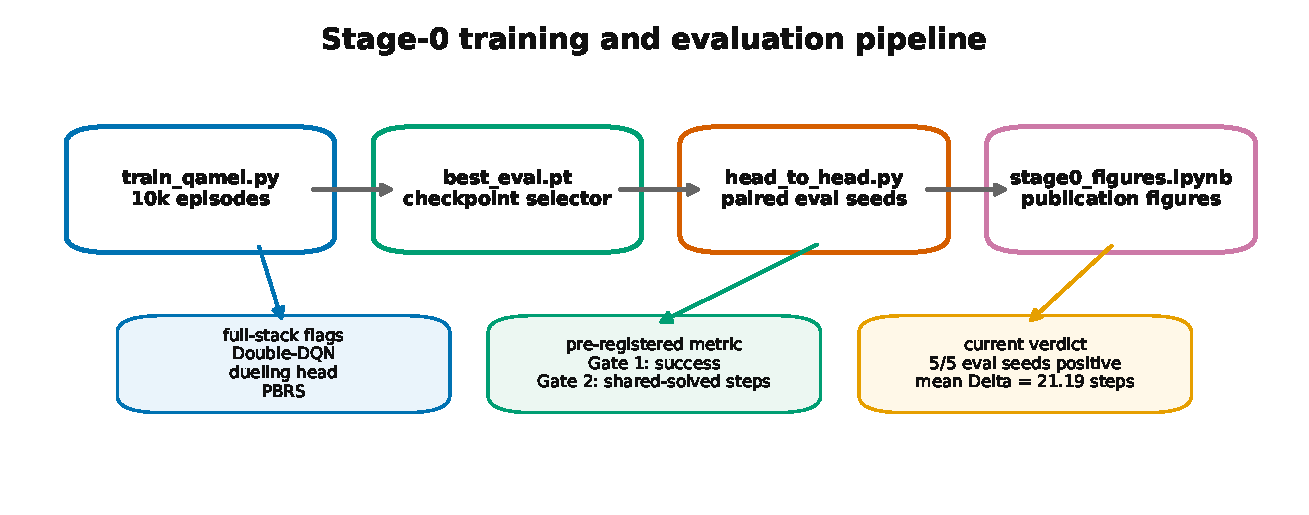
\includegraphics[width=0.98\textwidth]{figures/codeoverview_stage0_pipeline.pdf}
  \caption{Stage-0 pipeline. Training produces a \file{best\_eval.pt} checkpoint, the
  paired head-to-head harness evaluates the learned policy against the heuristic
  on identical stochastic instances, and \file{stage0\_figures.ipynb} turns the
  locked artifacts into publication figures.}
  \label{fig:stage0-pipeline}
\end{figure}

\subsection{Stage-0 method in one pass}
The full-stack Stage-0 configuration uses:
\begin{itemize}
  \item \code{counter\_exposed\_plus\_ready} observations: adjacency, generation counters, swap counters, and a derived swap-readiness channel.
  \item Dueling DQN: a shared trunk with separate value and advantage heads,
  \begin{equation*}
    Q(s,a)=V(s)+A(s,a)-\frac{1}{|\mathcal{A}|}\sum_{a'}A(s,a').
  \end{equation*}
  \item Double-DQN target updates: the policy network chooses the best valid next
  action while the target network evaluates that action.
  \item State-valid action masking both at acting time and inside the Bellman target.
  \item Potential-based reward shaping (PBRS) with
  \begin{equation*}
    F(s,s')=\gamma\Phi(s')-\Phi(s),
  \end{equation*}
  where $\Phi(s)$ is the longest contiguous run of elementary links starting at
  node~0. This is a learning aid, not a new physical evaluation metric.
  \item Correct separation of \code{terminated} and \code{truncated}: time-limit
  truncations continue to bootstrap, while true terminal states mask the target.
\end{itemize}

\subsection{Stage-0 physics in one pass}
The experiment models discrete control of a binary Bell-pair repeater chain. A
generation request samples a nearest-neighbour Bell pair with probability
$\pgen=0.4$; a swap request at an interior node samples entanglement swapping with
probability $\pswap=0.7$. A successful swap consumes two shorter links and creates
a longer link between their outer endpoints. The target event is a direct
end-to-end link between the two boundary nodes. The model does not simulate
fidelity, decoherence, finite memory lifetime, physical clock time, purification,
classical signaling, or grid/multipartite fusion. Therefore the Stage-0 claim is
about \emph{control efficiency in discrete repeater-chain scheduling}, not about
full physical latency.

\subsection{Stage-0 numerical result}
The head-to-head comparison follows the pre-registered metric in \file{METRIC.md}.
It evaluates \code{dqn\_greedy} and the non-neural prefer-swap-when-ready heuristic
on the same $1000$ stochastic episodes for each of five evaluation seeds:
$12345,23456,34567,45678,56789$.

The decision rule has two ordered gates. Gate~1 requires non-inferior success
relative to the heuristic within $\delta=0.02$. Gate~2 restricts to the
shared-solved episode set and computes
\begin{equation*}
  \Delta = \text{steps}_{\text{heuristic}} - \text{steps}_{\text{DQN}}.
\end{equation*}
A positive $\Delta$ means the DQN spans the same problem instance faster.

\begin{center}
\begin{tabular}{lr}
\toprule
Metric & Stage-0 value \\
\midrule
DQN greedy success rate & 0.9874 \\
Heuristic success rate & 0.8550 \\
DQN greedy mean steps & 17.2091 \\
Heuristic mean steps & 38.1017 \\
Shared-solved paired mean $\Delta$ & 21.1889 steps \\
95\% paired-$t$ CI for mean $\Delta$ & [20.2454,\;22.1325] \\
Positive evaluation seeds & 5/5 \\
Gate verdict & WIN \\
\bottomrule
\end{tabular}
\end{center}

\begin{figure}[htbp]
  \centering
  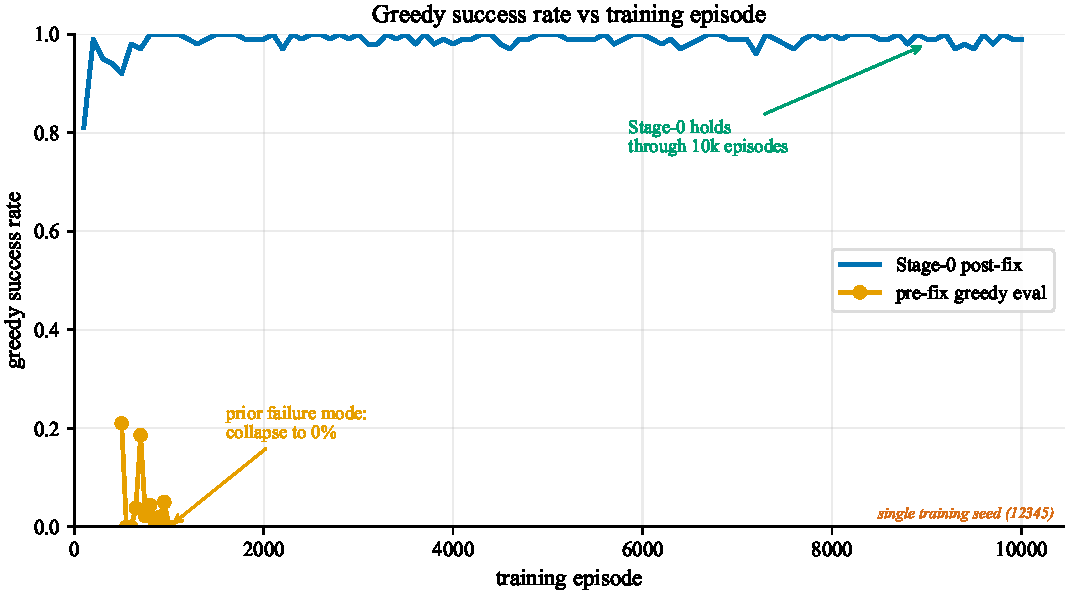
\includegraphics[width=0.93\textwidth]{figures/fig_stage0_collapse_fixed.pdf}
  \caption{The corrected Stage-0 training path removes the late greedy-evaluation
  collapse seen in the pre-fix checkpoint sweep. Both traces are plotted on the
  same greedy-success-rate axis.}
  \label{fig:stage0-collapse-fixed}
\end{figure}

\begin{figure}[htbp]
  \centering
  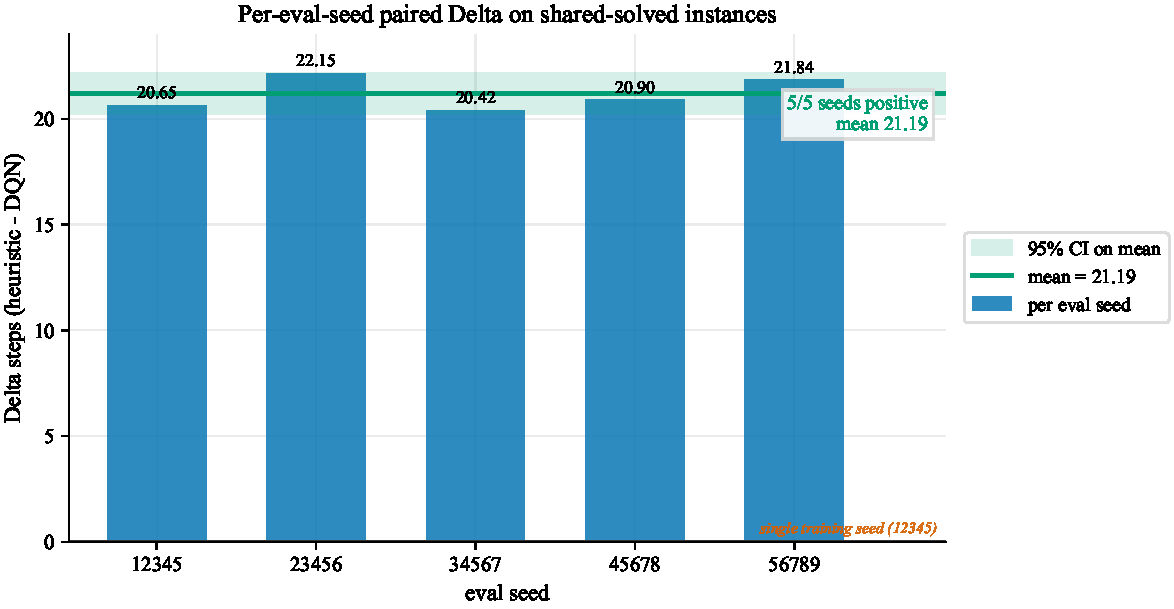
\includegraphics[width=0.90\textwidth]{figures/fig_stage0_paired_delta.pdf}
  \caption{Per-evaluation-seed paired step advantage. On the shared-solved
  episode intersections, all five evaluation seeds have positive
  $\Delta=\text{heuristic steps}-\text{DQN steps}$, with mean 21.19 steps.}
  \label{fig:stage0-paired-delta}
\end{figure}

\begin{figure}[htbp]
  \centering
  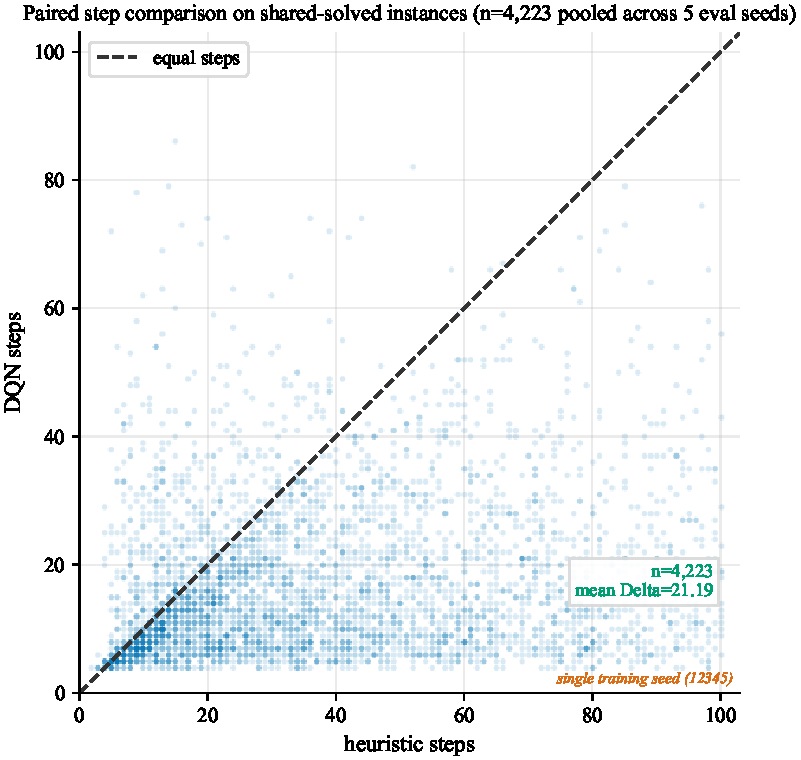
\includegraphics[width=0.92\textwidth]{figures/fig_stage0_paired_scatter.pdf}
  \caption{Episode-level paired scatter over the 4,223 pooled shared-solved
  instances. Points below the dashed $y=x$ diagonal are direct DQN step wins on
  identical stochastic problem instances.}
  \label{fig:stage0-paired-scatter}
\end{figure}

\begin{figure}[htbp]
  \centering
  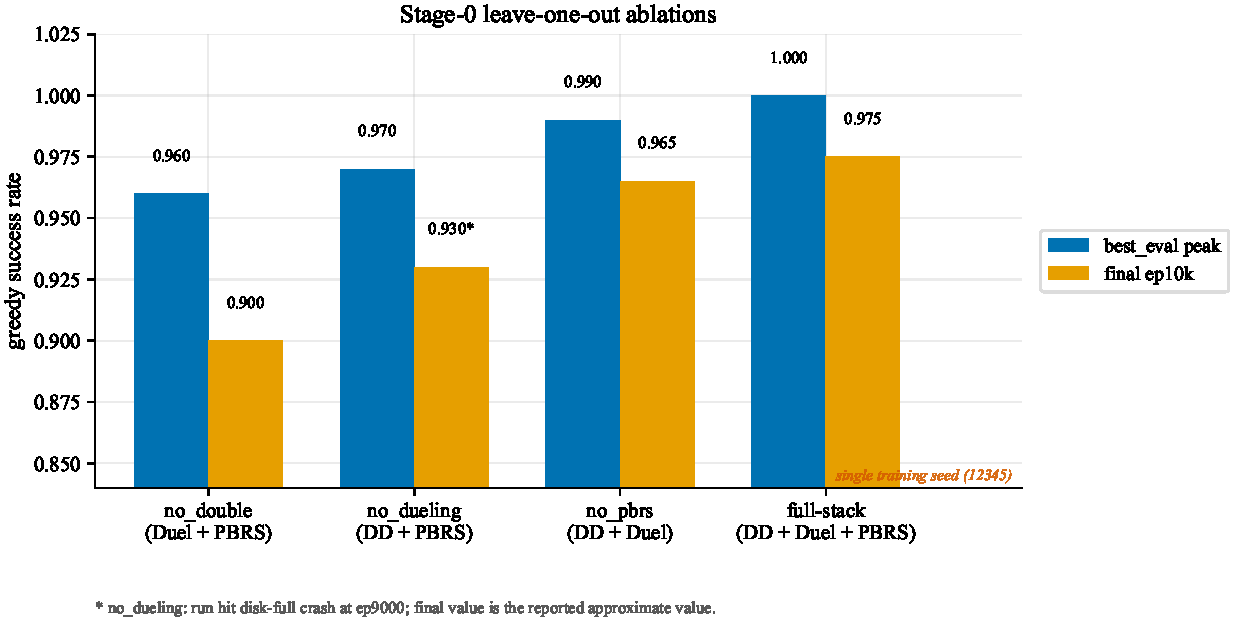
\includegraphics[width=0.90\textwidth]{figures/fig_stage0_ablation.pdf}
  \caption{Stage-0 leave-one-out ablations. Double-DQN is the largest stabilizer
  in this stack; dueling and PBRS add incremental value once the
  termination/truncation and target-masking fixes are in place.}
  \label{fig:stage0-ablation}
\end{figure}

\section{Project Overview and Scope}
\label{sec:overview}

\subsection{What the repository \emph{actually implements}}
The executable RL code learns a control policy for a \emph{one-dimensional quantum repeater chain}. It does not, at present, implement a 2D grid with multipartite (GHZ-class) distribution; that broader setting only appears in the analytical baseline files and in the OFC~2025 paper PDF (\file{OFC\_paper\_2025.pdf}).

\begin{figure}[htbp]
  \centering
  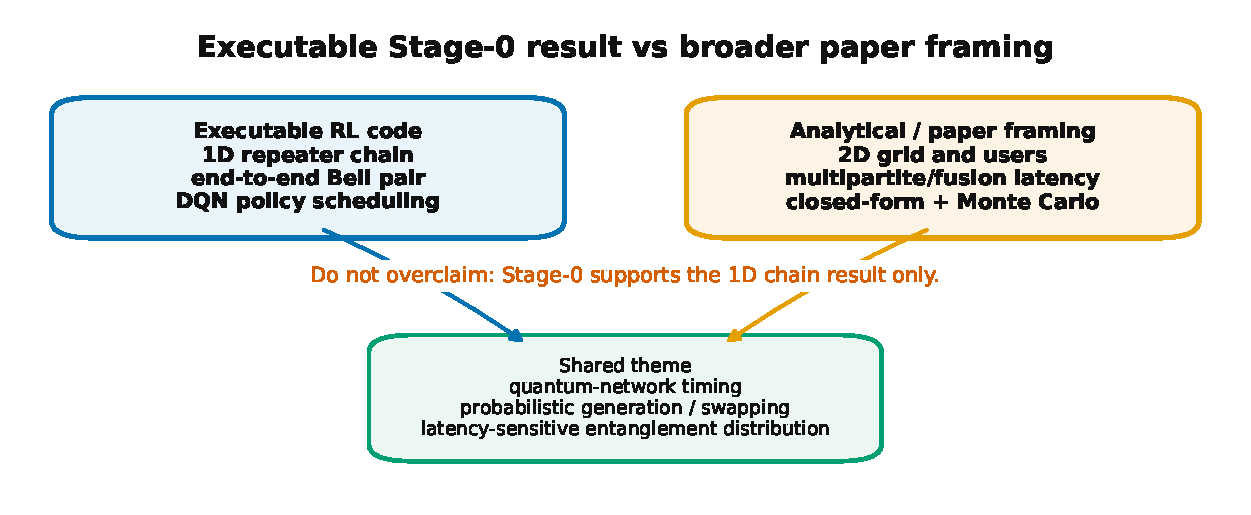
\includegraphics[width=0.98\textwidth]{figures/codeoverview_scope_map.pdf}
  \caption{Scope map for collaborators. The executable Stage-0 result supports
  the 1D repeater-chain Bell-pair scheduler. The grid/multipartite/fusion story
  is present in the analytical and paper-framing layer but is not yet an RL
  environment.}
  \label{fig:scope-map}
\end{figure}

Concretely:
\begin{itemize}
  \item A chain of $n$ nodes, indexed $0,1,\dots,n-1$. Nodes $0$ and $n-1$ are the endpoints. Interior nodes are repeaters.
  \item Nearest-neighbour elementary links $(i,i+1)$ can be probabilistically generated with success probability $\pgen$.
  \item Interior repeater nodes can attempt entanglement swapping, succeeding with probability $\pswap$.
  \item Goal: produce a direct entangled link between node $0$ and node $n-1$ using as few elementary operations / steps as possible.
\end{itemize}

The repository ships two RL solvers for this problem:
\begin{enumerate}
  \item A \textbf{tabular Q-learning} baseline (\file{qamel/agent.py}) over enumerated adjacency states. This scales to roughly $n \leq 6$.
  \item A \textbf{Deep Q-Network} (\file{qamel/dqn.py}, \file{scripts/train\_qamel.py}). This is the workhorse for $n \in \{5,6\}$ with curriculum learning.
\end{enumerate}

\subsection{What the analytical side implements (different problem!)}
The files in \file{analytical\_solution/} and the verification notebooks (\file{notebooks/verify\_simulations.ipynb}, \file{notebooks/calculate\_ratio\_and\_latencies.ipynb}) compute closed-form and Monte-Carlo waiting-time statistics for a \emph{grid topology} with four users at the corners and a central node. They include fusion probability $\pfusion$. These functions are not currently wired into the RL environment; they sit alongside it as a reference benchmark.

\subsection{Why the two scopes diverge}
The OFC~2025 paper frames the work as multipartite entanglement distribution in a quantum software-defined networking (SDN) architecture, including fusion and latency budgeting. The RL code is a strict subproblem: bipartite end-to-end Bell-pair scheduling on a chain. Any physics-aware reviewer must keep this divergence in mind. See \S\ref{sec:issues} for the canonical list of known mismatches.

\section{Physical Model}
\label{sec:physics}

\begin{figure}[htbp]
  \centering
  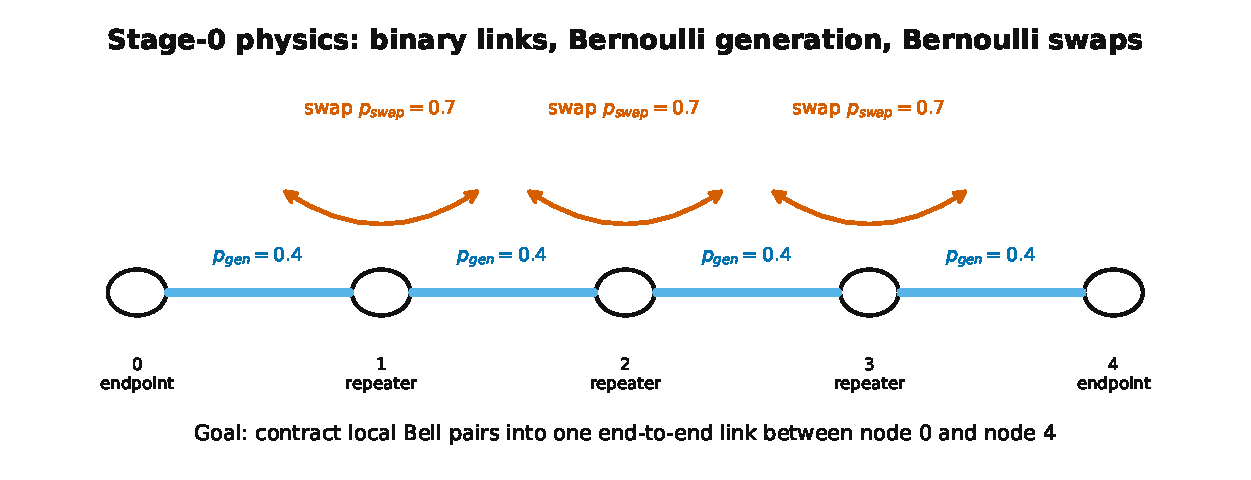
\includegraphics[width=0.98\textwidth]{figures/codeoverview_chain_physics.pdf}
  \caption{Physics abstraction used by Stage-0. The agent schedules elementary
  generation on nearest-neighbour segments and swaps at interior repeaters until
  the chain contracts into one end-to-end Bell pair.}
  \label{fig:chain-physics}
\end{figure}

\subsection{Chain dynamics implemented in \code{RepeaterChain}}
The class \code{RepeaterChain} (\file{qamel/environment.py:3}) is the entire executable physics model. It assumes:
\begin{description}[leftmargin=2.2em,style=nextline]
  \item[Topology] Linear chain of $n$ nodes; only nearest-neighbour elementary links are allowed.
  \item[Link representation] Binary; either an entangled link is present between two nodes or it is not. No fidelity, no Schmidt rank, no Werner parameter.
  \item[Generation] On an action requesting an elementary edge $(i,i+1)$, the existing link is cleared, both endpoint generation counters are incremented, and the link is re-sampled with $\Pr=\pgen$.
  \item[Swapping] On an action requesting a swap at interior node $k$ with exactly two currently-incident links (to neighbours $j$ and $\ell$), the swap counter at $k$ is incremented and with $\Pr=\pswap$ a direct edge $(j,\ell)$ is created. The two links incident to $k$ are then removed unconditionally.
  \item[Persistence] Links remain present until consumed by a swap or until the agent re-requests generation on that edge.
\end{description}

\subsection{What is intentionally \emph{not} modelled}
For a physics collaborator, the most important omissions are:
\begin{itemize}
  \item No memory lifetime / decoherence.
  \item No fidelity tracking. Entanglement is treated as ideal Bell pairs.
  \item No classical signaling latency. Each environment ``step'' is unitless.
  \item No teleportation latency or BSM duration.
  \item No fusion operations. (Fusion appears only in the analytical equations.)
  \item No noise model on swaps beyond the Bernoulli success/fail.
\end{itemize}
The exported metrics \code{ent\_attempt\_max} and \code{swap\_attempt\_max} are then post-processed by \file{notebooks/calculate\_ratio\_and\_latencies.ipynb} into physical latencies under fixed operation-time and fibre-propagation assumptions. That post-processing is external to the RL environment.

\section{MDP Formulation}
\label{sec:mdp}

\begin{figure}[htbp]
  \centering
  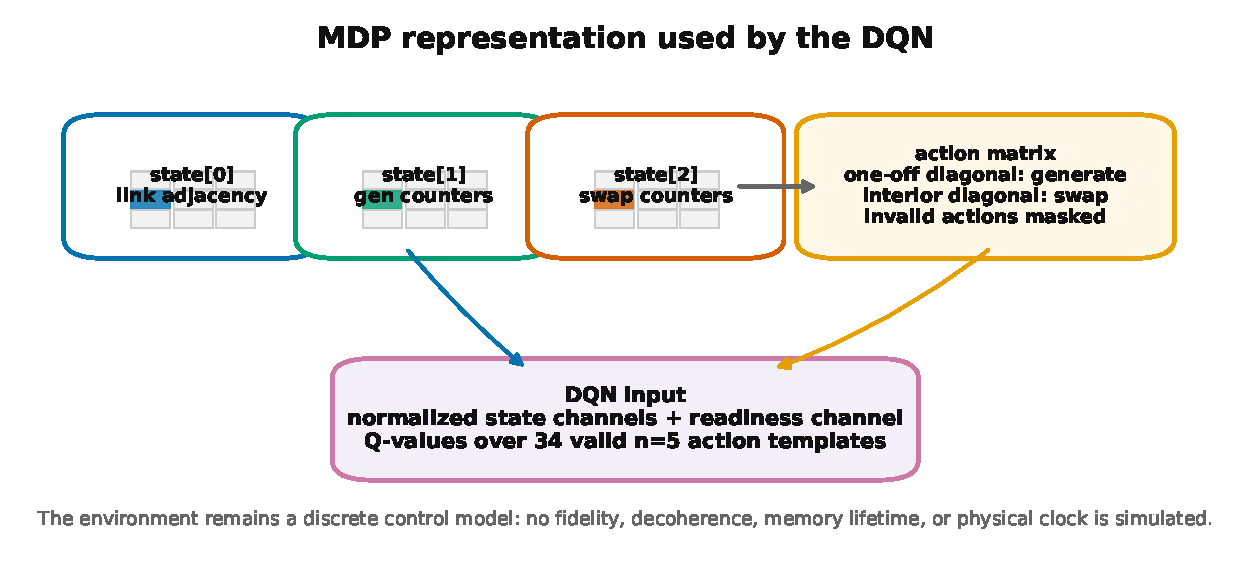
\includegraphics[width=0.98\textwidth]{figures/codeoverview_mdp_state_action.pdf}
  \caption{MDP representation. The physical state is stored as three
  $n\times n$ channels; Stage-0 adds a derived readiness channel before feeding
  the observation to the DQN. The action is also an $n\times n$ matrix, with
  generation encoded on one-off diagonals and swaps encoded on interior diagonal
  entries.}
  \label{fig:mdp-state-action}
\end{figure}

\subsection{State $s_t \in \mathbb{R}^{3 \times n \times n}$}
\code{RepeaterChain.reset()} returns a $3\times n\times n$ zero tensor (\file{qamel/environment.py:10}). The three channels are:
\begin{center}
\begin{tabular}{cl}
\toprule
Channel & Meaning \\
\midrule
$s[0]$ & Symmetric binary adjacency matrix of current entangled links. \\
$s[1]$ & Diagonal-only: per-node \emph{generation attempt} counter. \\
$s[2]$ & Diagonal-only: per-node \emph{swap attempt} counter. \\
\bottomrule
\end{tabular}
\end{center}
Counter channels are populated only on the diagonal. The off-diagonals of $s[1]$ and $s[2]$ remain zero throughout an episode.

\subsection{Action $a_t \in \{0,1\}^{n \times n}$}
An action is itself an $n \times n$ binary matrix encoding two simultaneous decisions:
\begin{itemize}
  \item \textbf{Generation requests}: the one-offset diagonals $a[i,i+1]$ (and symmetrically $a[i+1,i]$) mark which elementary edges should be attempted this step. A generation request can ``refresh'' an existing link (clear it and re-sample).
  \item \textbf{Swap requests}: the diagonal entries $a[k,k]$ for interior nodes $k \in \{1,\dots,n-2\}$ mark which repeater nodes should attempt a swap.
\end{itemize}
A \emph{no-op} action is the zero matrix; it advances the step counter but does not touch the chain.

The complete set of admissible actions is enumerated once per $n$ by \code{generate\_all\_valid\_actions} (\file{qamel/utils.py}):
\begin{enumerate}
  \item Form all matrices with arbitrary interior-diagonal and one-offset-diagonal bits, forcing endpoint diagonals to zero. There are $2^{(n-2)+(n-1)}$ such candidates (\file{qamel/utils.py}).
  \item Reject any matrix where the row/column of a swap-marked node is nonzero off the diagonal. This enforces ``do not generate a new edge on a node that you are also swapping this step.''
\end{enumerate}
Measured action-set cardinalities:
\begin{center}
\begin{tabular}{rr}
\toprule
$n$ & $|\mathcal{A}_{\text{valid}}|$ \\
\midrule
3 & 5 \\
4 & 13 \\
5 & 34 \\
6 & 89 \\
7 & 233 \\
\bottomrule
\end{tabular}
\end{center}

\subsection{Transition $P(s_{t+1}\mid s_t, a_t)$}
The transition is implemented as a single Python method, \code{RepeaterChain.step} (\file{qamel/environment.py:14}). In pseudocode:
\begin{verbatim}
clone state s -> s'

for each upper-triangular edge (i,j) with a[i,j]=1:
    s'[1][i,i] += 1                   # generation counter at i
    s'[1][j,j] += 1                   # generation counter at j
    s'[0][i,j] = s'[0][j,i] = 0       # clear edge
    if Bernoulli(pgen) succeeds:
        s'[0][i,j] = s'[0][j,i] = 1   # success creates the link

for each interior k with a[k,k]=1:
    neighbours = nonzero indices of s'[0][k]
    if len(neighbours) > 2:
        return (-100, s')             # ill-typed early exit (see issues)
    if len(neighbours) == 2:
        s'[2][k,k] += 1
        let (j, l) = neighbours
        carry = max(s'[0][j,k], s'[0][l,k])  # always 1 here
        if Bernoulli(pswap) succeeds:
            s'[0][j,l] = s'[0][l,j] = carry
        s'[0][j,k] = s'[0][k,j] = 0
        s'[0][l,k] = s'[0][k,l] = 0

return s'
\end{verbatim}
Two subtle points:
\begin{itemize}
  \item Generation requests are processed \emph{before} swap requests, so a freshly generated link could in principle be swapped within the same step. However, \code{generate\_all\_valid\_actions} forbids actions that simultaneously generate and swap at the same node, so the chain semantics are well defined.
  \item The branch on \code{len(neighbours) > 2} returns a tuple instead of a tensor. This is a latent bug (see \S\ref{sec:issues}, item~13).
\end{itemize}

\subsection{Terminal conditions}
Defined in \file{qamel/utils.py}:
\begin{itemize}
  \item \textbf{Final / successful}: \code{check\_if\_final\_state} (\file{qamel/utils.py}) returns true when $s[0,n-1] \ne 0$.
  \item \textbf{Bad}: \code{check\_if\_bad\_state} (\file{qamel/utils.py}) returns true when any endpoint has degree $> 1$ or any interior node has degree $> 2$.
  \item \textbf{Truncated}: episode length reached \code{max\_actions} (default 100).
\end{itemize}
\code{get\_episode\_status} (\file{qamel/utils.py}) is the canonical reducer: it considers a state ``final'' only if it is final \emph{and not} simultaneously bad.

\subsection{Reward}
The reward is implemented in \code{reward\_shape} and wrapped by \code{compute\_reward} (\file{qamel/utils.py}):
\begin{equation*}
r_t = \begin{cases}
+100 & \text{if terminated (final and not bad)} \\
-100 & \text{if bad or truncated} \\
-1   & \text{otherwise}
\end{cases}
\end{equation*}
Currently \code{reward\_mode="base"} is the only supported mode; the function signature contains \code{swap\_ready\_bonus} for backward compatibility, but the bonus is not applied in the current canonical reward path.

\paragraph{Historical note.} The original \code{REPORT.md} describes a terminal reward of $1000/\max(s)$ and a separate training-time \code{swap\_ready\_bonus}. Both have since been removed in favour of the simpler $\pm 100/-1$ scheme shown above. The codebase still exposes the \code{--swap\_ready\_bonus} flag for command-line compatibility, but \code{compute\_reward} now ignores it.

\subsection{Valid-action mask}
\code{is\_action\_valid\_given\_state} (\file{qamel/utils.py}) computes a state-conditional validity check used both during action selection and during DQN target backups:
\begin{enumerate}
  \item For each requested new edge in the upper triangle, increment a hypothetical post-action degree at each endpoint.
  \item Endpoints have a hard cap of 1; interior nodes have a cap of 2.
  \item Additionally, any node marked for swap must end up with post-action degree exactly 2 (otherwise the swap is meaningless or invalid).
\end{enumerate}
This is a more refined check than the structural \code{generate\_all\_valid\_actions} step: it depends on the current state, not just on the action layout.

\section{The Reinforcement Learning Code}
\label{sec:rl}

\subsection{Tabular Q-learning (baseline)}
File: \file{qamel/agent.py}. The \code{Agent} class:
\begin{itemize}
  \item Enumerates all valid adjacency states via \code{generate\_all\_valid\_states} (\file{qamel/utils.py}). Caches them under \file{qamel/outputs/logs/states/\{n\}\_nodes.npy}.
  \item Enumerates all valid actions and caches them under \file{qamel/outputs/logs/actions/\{n\}\_nodes.npy}. These are also reused by the DQN code.
  \item Holds a $|\mathcal{S}_{\text{valid}}| \times |\mathcal{A}_{\text{valid}}|$ Q-table.
  \item Exploration in \code{predict\_action} (\file{qamel/agent.py:50}) is intended to be $\varepsilon$-greedy but currently uses \code{torch.randn(1) < epsilon} --- a standard-normal comparison rather than a uniform one. This is a known bug.
  \item Terminal update in \code{update\_q\_table} (\file{qamel/agent.py:60}) adds $Q$ instead of subtracting it, which is also incorrect.
\end{itemize}
For physics-side collaboration this learner can be treated as a smoke-test only; the real benchmark is the DQN.

\subsection{DQN: observation modes}
File: \file{qamel/dqn.py}. \code{preprocess\_obs(state, obs\_mode, counter\_norm)} produces the network input.

\begin{center}
\begin{tabular}{lll}
\toprule
\code{obs\_mode} & Tensor shape & Contents \\
\midrule
\code{baseline} & $(n,n)$ & Adjacency only (used by tabular learner). \\
\code{counter\_exposed} & $(3,n,n)$ & Adjacency + normalised gen/swap counters. \\
\code{counter\_exposed\_plus\_ready} & $(4,n,n)$ & The above + global swap-readiness channel. \\
\bottomrule
\end{tabular}
\end{center}
The counter normalisation clamps $s[1], s[2]$ to $[0,1]$ after dividing by \code{counter\_norm} (default 20). The swap-readiness channel is a constant plane equal to the count of interior nodes with current degree 2, providing a coarse ``ready to swap somewhere'' signal that survives convolution-free preprocessing.

\subsection{DQN: network}
\code{DQNNet} (\file{qamel/dqn.py}) is the default flat MLP:
\begin{verbatim}
Flatten -> Linear(input, H) -> ReLU
       -> Linear(H, H)       -> ReLU
       -> Linear(H, |A|)
where H = max(512, ceil(4 * input / 256) * 256)
\end{verbatim}
The hidden width formula scales with the flattened observation dimension. For $n=5$, \code{counter\_exposed\_plus\_ready} has input dim $100$, so $H=512$. For $n=6$ the input dim is $144$ and the formula yields $H=768$ (since $4\times144=576$ rounds up to the next 256-multiple, $768$).

\code{DuelingDQNNet} is also available through \code{build\_dqn\_net(..., net\_arch="dueling")} and through the training flag \code{--dueling}. It uses the same flatten/two-layer trunk and then separate value and advantage heads:
\begin{equation*}
Q(s,a) = V(s) + A(s,a) - \frac{1}{|\mathcal{A}|}\sum_{a'} A(s,a').
\end{equation*}
The trunk is intentionally named \code{net.1} and \code{net.3}, matching \code{DQNNet}'s first two linear layers. This allows partial trunk-weight transfer from a plain DQN checkpoint into a dueling checkpoint by matching state-dict keys; only the final plain-DQN output layer is architecture-specific.

\subsection{DQN: training loop}
The full DQN training loop is in \code{train\_dqn\_agent} (\file{scripts/train\_qamel.py:558}). The structure, in order:
\begin{enumerate}
  \item Build \code{RepeaterChain} environment.
  \item Load (or generate and cache) the enumerated valid-action tensor.
  \item Identify the no-op action index for fallback.
  \item Build policy and target networks (\code{DQNNet} or \code{DuelingDQNNet}), Adam optimiser, replay buffer.
  \item Optionally restore from a checkpoint (\code{resume\_checkpoint}) including replay buffer, RNG state, optimiser state, and episode-level metric arrays.
  \item Episode loop:
    \begin{enumerate}
      \item Optionally adjust the per-episode action horizon via the curriculum (see \S\ref{sec:curriculum}).
      \item At each step:
        \begin{itemize}
          \item Compute the linear $\varepsilon$ from \code{linear\_schedule} (\file{qamel/utils.py}).
          \item Compute valid action indices for the current state.
          \item Optionally restrict to swap-only actions when at least one interior node is swap-ready and \code{--prefer\_swap\_when\_ready\_train} is set.
          \item $\varepsilon$-greedy choice over the restricted index set, with invalid Q-values masked to $-10^9$.
          \item Step the environment, compute unshaped environment reward via \code{compute\_reward}.
          \item If \code{--pbrs} is enabled, compute $F=\gamma\Phi(s')-\Phi(s)$ and push $r_{\text{train}}=r_{\text{env}}+\lambda F$ into replay, where $\lambda$ is \code{pbrs\_scale}. Episode metrics still use $r_{\text{env}}$.
          \item Push transition into the replay buffer (CPU tensors), storing \code{terminated} and \code{truncated} separately.
          \item If buffer is large enough, sample a batch, build the Bellman target, mask next-state invalid actions \emph{too} (\code{\_build\_valid\_action\_mask}, \file{scripts/train\_qamel.py}), compute Smooth-L1 (Huber) loss, optimise with gradient clipping at $\|g\| \le 10$. If \code{--double-dqn} is enabled, the policy net selects the next action and the target net evaluates it.
          \item Periodically refresh the target network from the policy network.
        \end{itemize}
      \item At end of episode: record return, steps, success flag, mean per-step loss, mean swap-readiness.
      \item Optionally save a checkpoint at \code{--checkpoint\_every}, emit a metrics row at \code{--log\_every}.
      \item Optionally run an offline ``best-eval'' rollout (\S\ref{sec:besteval}) and update the best-eval checkpoint if the snapshot beats the running best on $(\text{success rate}, \text{mean return}, \text{lower mean steps})$ lex order.
    \end{enumerate}
  \item Return the final tuple of (policy net, target net, optimiser, replay buffer, episode arrays, global step count, completed episodes, best-eval metrics).
\end{enumerate}

\subsection{DQN hyperparameters (canonical)}
From \code{dqn\_hyperparameters} (\file{scripts/train\_qamel.py:79}):
\begin{center}
\begin{tabular}{lr}
\toprule
Parameter & Value \\
\midrule
$\gamma$ (discount) & 0.99 \\
Learning rate & $10^{-3}$ \\
Batch size & 64 \\
Replay buffer capacity & 50{,}000 \\
Target network update period (env steps) & 1{,}000 \\
$\varepsilon_{\text{start}}$ & 1.0 \\
$\varepsilon_{\text{end}}$ & 0.05 \\
$\varepsilon$-decay steps & 10{,}000 \\
Counter normalisation $c_{\text{norm}}$ & 20.0 \\
Loss & Smooth-L1 (Huber) \\
Optimiser & Adam \\
Grad clip & $\|g\|_2 \le 10$ \\
\bottomrule
\end{tabular}
\end{center}

The CLI can override the learning rate and batch size with \code{--lr} and \code{--batch\_size}. Architecture and target-update variants are controlled by \code{--dueling} and \code{--double-dqn}; reward shaping is controlled by \code{--pbrs} and \code{--pbrs-scale}.

\subsection{Curriculum learning}
\label{sec:curriculum}
With \code{--use\_curriculum}, the training loop divides the episode budget into three phases by \code{--curriculum\_boundaries} (default $5{,}000;\;10{,}000$) and uses progressively larger per-episode action horizons from \code{--curriculum\_steps} (default $20,40,100$). Each time the phase rolls over, a one-line status print announces the new horizon.

\subsection{Best-eval checkpointing}
\label{sec:besteval}
When \code{--best\_eval\_every} $> 0$, every $k$ episodes the training loop:
\begin{enumerate}
  \item Snapshots the RNG state.
  \item Reseeds with \code{--best\_eval\_seed}.
  \item Switches the policy net to eval mode and runs \code{--best\_eval\_episodes} rollouts at $\varepsilon=0$, masking invalid actions but \emph{not} applying the prefer-swap-when-ready filter.
  \item Computes (success\_rate, timeout\_rate, mean\_return, mean\_steps, mean\_ent\_attempt\_max, mean\_swap\_attempt\_max).
  \item If the lexicographic comparator \code{\_is\_better\_eval\_metrics} prefers the candidate, the best-eval checkpoint and JSON are updated.
  \item Restores the prior RNG state to avoid biasing the training stochastics.
\end{enumerate}
This is the primary path for ``frozen, reproducible'' policy selection during long runs.

\subsection{Resume semantics}
\label{sec:resume}
On startup the training script searches for, in this order, the latest checkpoint at\\\file{qamel/outputs/runs/\textless run\_name\textgreater/checkpoints/latest.pt}, then a legacy checkpoint location, then the final model file. If a checkpoint is found and \code{--force\_train} is \emph{not} set, training resumes from it: model weights, optimiser state, replay buffer contents, RNG state, episode arrays, and the global step count are all restored. The validator \code{\_validate\_resume\_checkpoint} (\file{scripts/train\_qamel.py}) refuses to resume if $n$, $\pgen$, $\pswap$, \code{obs\_mode}, \code{reward\_mode}, \code{swap\_ready\_bonus}, \code{prefer\_swap\_when\_ready\_train}, \code{seed}, or \code{net\_arch} differ from those baked into the checkpoint.

\section{Evaluation Pipeline}
\label{sec:eval}

The script \file{scripts/evaluate\_qamel.py} is the canonical offline checkpoint benchmark. It builds the network through \code{build\_dqn\_net}, so checkpoints with \code{net\_arch="dqn"} and \code{net\_arch="dueling"} are both loadable.

\subsection{Policy execution}
For each evaluation episode:
\begin{itemize}
  \item Reset the environment.
  \item Loop steps until terminal/truncated.
  \item At each step, compute the validity mask, optionally apply ablation filters (\S\ref{sec:ablations}), choose an action greedily (or $\varepsilon$-soft if \code{--eval\_epsilon} $>0$), step the environment, accumulate reward.
  \item Record episode-level statistics.
\end{itemize}

\subsection{Ablation filters}
\label{sec:ablations}
Three filters can be combined on the valid-action set:
\begin{description}[leftmargin=2em]
  \item[\code{--mask\_null\_action}] Forbids the no-op when other actions are valid.
  \item[\code{--block\_refresh\_actions}] Disallows actions whose generation requests overlap a currently-active edge. This prevents the policy from ``wasting'' a generation attempt to refresh a link that is already up.
  \item[\code{--prefer\_swap\_when\_ready}] If any interior node has post-action degree 2 (i.e.\ is ready to swap), restrict the candidate set to actions that include at least one swap bit.
\end{description}
If filtering reduces the set to empty, the loop transparently falls back to the unfiltered valid-action set and increments \code{ablation\_empty\_fallbacks} in the summary JSON, so the experimenter can detect when ablations are being silently ignored.

\subsection{Tracing}
With \code{--trace\_max\_episodes} $>0$, a structured per-step JSON trace is emitted. Each step records: pre-state summary (active links, swap-ready node count, ent/swap attempt maxima), action summary (generation edges, swap nodes, refresh edges, null-action flag), reward, post-state summary, and status flags. With \code{--trace\_failed\_only} the trace is filtered to episodes that did not end in a successful final state. The trace lives at \code{--trace\_output\_path}.

\subsection{Artifacts}
For each evaluation invocation the script writes:
\begin{itemize}
  \item \file{qamel/outputs/runs/\textless run\_name\textgreater/evaluations/\textless eval\_name\textgreater.csv} (per-episode rows).
  \item \file{...\_summary.json} with the aggregate metrics.
  \item \file{...\_ent\_counts.txt}, \file{...\_swap\_counts.txt} for the count distributions.
  \item A legacy global CSV \file{qamel/outputs/results/eval\_n\textless n\textgreater\_pgen\textless p\textgreater\_pswap\textless q\textgreater\_\textless tag\textgreater.csv} for backwards compatibility with the notebooks.
\end{itemize}
The \code{run\_name} is built deterministically as \code{dqn\_n\textless n\textgreater\_pgen\textless p\textgreater\_pswap\textless q\textgreater\_\textless tag\textgreater}; \code{eval\_name} is \code{eval\_episodes\textless E\textgreater\_max\textless M\textgreater\_eps\textless eps\textgreater\_seed\textless s\textgreater} when a seed is supplied.

\subsection{Head-to-head policy comparison}
\file{scripts/head\_to\_head.py} compares three policies on the same environment configuration read from a run directory's \file{config.json}:
\begin{description}[leftmargin=2em]
  \item[\code{dqn\_greedy}] DQN argmax over the state-conditional valid-action mask, with no prefer-swap filter.
  \item[\code{dqn\_swapprefer}] The same network, but if an interior node is currently degree 2, it restricts valid actions to those swapping at least one ready node; if the restriction is empty it falls back to the full valid set.
  \item[\code{heuristic}] No network. If a ready interior node exists, choose uniformly among valid actions that swap a ready node. Otherwise choose uniformly among valid generation-only actions, avoiding the null action unless forced.
\end{description}
For each policy and seed it records success rate, mean steps on successful episodes, mean return, truncated fraction, and success count. The JSON output contains \code{config}, \code{per\_run}, \code{summary}, and \code{verdict}. The \code{BEAT} verdict requires the mean greedy-DQN success rate to exceed the heuristic mean and at least four positive paired seed deltas under the default five-seed protocol.

\section{Multi-Budget Study Pipeline}
\label{sec:stage2}

The script \file{scripts/run\_stage2\_study.sh} is the canonical sweep driver for cluster (UCL Myriad) runs.

\subsection{Inputs (environment variables)}
\code{N, PGEN, PSWAP, OBS\_MODE, REWARD\_MODE, EVAL\_EPISODES, MAX\_ACTIONS, EVAL\_EPSILON, SEED, RUN\_TAG, BUDGETS, CHECKPOINT\_EVERY, LOG\_EVERY, BEST\_EVAL\_EVERY, BEST\_EVAL\_EPISODES, BEST\_EVAL\_MAX\_ACTIONS, BEST\_EVAL\_SEED, COUNTER\_NORM, SWAP\_READY\_BONUS, PREFER\_SWAP\_WHEN\_READY\_TRAIN, USE\_CURRICULUM, STUDY\_ROOT, ALLOW\_ARCHIVE\_OVERWRITE, STUDY\_FORCE\_TRAIN}. Defaults match the canonical phase-2 preset.

\subsection{Loop structure}
For each budget $B$ in \code{BUDGETS} (default $10000, 50000, 100000, 200000$):
\begin{enumerate}
  \item Refuse to overwrite a non-empty archive directory unless \code{ALLOW\_ARCHIVE\_OVERWRITE=1}.
  \item Call \file{train\_qamel.py} with \code{--train\_episodes=B}. Because of the resume logic, this picks up where the previous budget left off (so $50000$ is an additional $40000$ episodes after $10000$, not from scratch). \code{STUDY\_FORCE\_TRAIN=1} only injects \code{--force\_train} when the run directory does not yet exist.
  \item Call \file{evaluate\_qamel.py} at that budget.
  \item Assert that all the expected artifacts exist.
  \item Copy them under \file{qamel/outputs/studies/\textless RUN\_TAG\textgreater/budget\_\textless B\textgreater/}.
  \item Rebuild \file{cross\_budget\_summary.csv} from the archived JSON summaries.
\end{enumerate}

\subsection{Cross-budget summary}
The CSV columns are: \code{budget, success\_rate, mean\_return, mean\_steps, mean\_ent\_attempt\_max, mean\_swap\_attempt\_max, truncated\_fraction}. This is the main quantitative deliverable of a stage-2 study.

\section{Analytical and Monte-Carlo Baseline}
\label{sec:analytic}

The directory \file{analytical\_solution/} contains a self-contained \emph{grid-topology} model used for paper figures and notebook verification. It is not currently coupled to the RL environment.

\subsection{\code{generate\_tpm(N, p, a)} (\file{analytical\_solution/analytical\_equations.py:4})}
Builds a transition probability matrix for an $N$-segment chain by recursive Kronecker doubling, following Shchukin et al.\ For each segment, the elementary TPM is
\begin{equation*}
T_1 = \begin{pmatrix} 1-p & p \\ 0 & 1 \end{pmatrix},
\end{equation*}
i.e.\ a Bernoulli generation per time step with absorbing ``link present'' state. The recursion repeatedly takes Kronecker products of pairs and applies a swap-failure redistribution:
\begin{equation*}
T_{2k}[:-1, 0] \mathrel{+}= (1-a)\, T_{2k}[:-1, -1], \qquad T_{2k}[:-1, -1] \mathrel{*}= a,
\end{equation*}
where $a \in \{\pswap, \pfusion\}$ depending on the caller. This implements ``swap fails $\Rightarrow$ restart both halves'' as a single absorbing step.

\subsection{\code{shchukin\_eq(n, p, a)}}
Returns the expected number of generation attempts to produce an entangled link spanning $n$ segments using the standard fundamental-matrix identity
\begin{equation*}
\bar K = (I - Q)^{-1} \mathbf{1},
\end{equation*}
where $Q$ is the substochastic block of $T$.

\subsection{\code{bernardes\_eq(n\_segments, p)}}
Implements the Bernardes closed form for non-deterministic generation:
\begin{equation*}
E[T] = \sum_{j=1}^{n}(-1)^{j+1} \binom{n}{j}\frac{1}{1-(1-p)^j}.
\end{equation*}
Valid only when generation is the rate-limiting step (no swap retries).

\subsection{\code{markov\_approach(vertices, p, a)} and \code{including\_fusion(vertices, p, a, f)}}
These specialise to a $V \times V$ grid with users at the four corners and a central node. The maximum Manhattan distance to the central node is computed, and \code{shchukin\_eq} (or its fusion-corrected variant) is evaluated at that distance. This is the analytical waiting-time model used in the paper figures.

\subsection{\code{n\_segment\_solution(n, pgen, pswap)}}
Returns the full vector $\bar K$ over all initial sub-states of an $n$-segment chain TPM. Useful when one wants the conditional expectations starting from a partially-built chain.

\subsection{Monte-Carlo sampler (\file{analytical\_solution/monte\_carlo.py})}
\code{MonteCarloFusion} samples waiting times by recursively realising the nested-swap tree:
\begin{itemize}
  \item Level 0: \code{np.random.geometric(pgen)} for an elementary link.
  \item Level $n>0$: sample two level-$(n-1)$ subtrees, take the max (both halves must be ready), increment the swap counter \code{tq}, and either accept with $\Pr=\pswap$ or recursively retry both halves.
  \item Fusion is applied multiplicatively: a separate geometric-distributed fusion attempt count is averaged in via \code{sample\_fusion}.
\end{itemize}
The top-level helper \code{monte\_carlo} returns the four-user joint waiting-time samples using the grid distances computed by \code{decompose\_into\_powers} (\file{analytical\_solution/utils.py:28}).

\subsection{Utility helpers (\file{analytical\_solution/utils.py})}
\code{manhattan\_distance}, \code{largest\_power\_of\_2}, \code{decompose\_into\_powers}, \code{normalize\_array}, plus \code{monte\_carlo\_sim} which is a thin wrapper for batched waiting-time sampling with a rich progress bar.

\section{Configuration and Canonical Baselines}
\label{sec:config}

\subsection{Phase-2 baseline ($n=5$)}
The canonical preset is \file{configs/phase2\_baseline\_n5\_plus\_ready.json}:
\begin{lstlisting}[language=]
{
  "name": "phase2_baseline_n5_plus_ready",
  "train": {
    "n": 5, "pgen": 0.4, "pswap": 0.7,
    "obs_mode": "counter_exposed_plus_ready",
    "seed": 12345, "reward_mode": "base",
    "swap_ready_bonus": 0.5,
    "train_episodes": 10000, "max_actions": 100,
    "checkpoint_every": 1000, "log_every": 100,
    "use_curriculum": false
  },
  "evaluate": {
    "eval_episodes": 500, "max_actions": 100, "eval_epsilon": 0.0
  }
}
\end{lstlisting}
The corresponding \file{BASELINE.md} pins this as the benchmark preset and documents the exact train/evaluate invocations.

\subsection{Reported result and current Myriad archive state}
\code{README.md} reports the following result on this preset, now confirmed in
the Myriad archive for the single-seed progressive $n=5$ run:
\begin{center}
\begin{tabular}{rrrl}
\toprule
$n$ & Budget & Success rate & Lab status \\
\midrule
5 & 10{,}000 & 90.4\% & archived and confirmed \\
5 & 20{,}000 & -- & started, checkpointed at 11{,}000, no archived eval \\
6 & 4{,}000 & 0.0\% & archived old progressive run \\
6 & 5{,}000+ & -- & later resume failed from checkpoint-width mismatch \\
\bottomrule
\end{tabular}
\end{center}
These are the numbers cited at submission time plus the June 17, 2026 Myriad
status. Larger $n=5$ budgets and any fresh $n=6$ claim still require clean
resubmission after the cluster checkout is updated.

\subsection{Myriad / qsub wrappers}
\file{scripts/myriad\_stage2\_lq\_seed12345\_progressive.sh}, \file{...\_n5...}, \file{...\_n6...intermediate.sh}, \file{...\_n6...progressive.sh}, and \code{qsub\_*} variants are minor wrappers around \file{run\_stage2\_study.sh} that set module loads, environment activation, and SGE qsub flags before delegating.

\section{Output Layout}
\label{sec:outputs}

Per training run:
\begin{verbatim}
qamel/outputs/runs/<run_name>/
  config.json
  model.pt                     # final model + full training state
  train.log
  metrics.csv                  # per-window training metrics
  checkpoints/
    latest.pt                  # the most recent checkpoint
    episode_000NNN.pt          # periodic checkpoints
    best_eval.pt               # best-eval policy snapshot
    best_eval_metrics.json
  evaluations/
    eval_episodes<E>_max<M>_eps<e>_seed<s>.csv
    eval_episodes<E>_max<M>_eps<e>_seed<s>_summary.json
    eval_episodes<E>_max<M>_eps<e>_seed<s>_ent_counts.txt
    eval_episodes<E>_max<M>_eps<e>_seed<s>_swap_counts.txt
\end{verbatim}
Shared caches:
\begin{verbatim}
qamel/outputs/logs/states/<n>_nodes.npy
qamel/outputs/logs/actions/<n>_nodes.npy
\end{verbatim}
Legacy locations (the codebase still writes to these for notebook compatibility):
\begin{verbatim}
qamel/outputs/models/dqn_n<n>_pgen<p>_pswap<q>_<tag>.pt
qamel/outputs/results/eval_n<n>_pgen<p>_pswap<q>_<tag>.csv
qamel/outputs/results/ent_counts/<n>_nodes.txt
qamel/outputs/results/swap_counts/<n>_nodes.txt
qamel/q_table_storage/<n>_nodes.txt
\end{verbatim}
Study archives:
\begin{verbatim}
qamel/outputs/studies/<RUN_TAG>/
  budget_<B>/
    model.pt, latest.pt, metrics.csv, train.log, config.json
    eval.csv, eval_summary.json
    best_eval.pt, best_eval_metrics.json   # if best-eval was enabled
  cross_budget_summary.csv
\end{verbatim}

\section{Known Issues and Modeling Caveats}
\label{sec:issues}

This list is distilled from \file{REPORT.md} and from the code itself. Items 1--3 are scientific in nature and require physics judgment to resolve; items 4+ are implementation defects.

\begin{enumerate}
  \item \textbf{Scope mismatch.} The RL code models a 1D chain producing a bipartite end-to-end Bell pair, while the README, the analytical files, and the OFC paper describe a 2D grid multipartite GHZ distribution with fusion. Until this is reconciled, any physics-aware contribution should declare which problem it is targeting.
  \item \textbf{No fidelity / decoherence / memory lifetime.} The environment is purely combinatorial. A realistic physics extension would add per-edge fidelity, a decay law $F(t)$ between attempts, and a memory-cutoff truncation rule.
  \item \textbf{Latency is not part of the MDP.} \code{step()} carries no physical time. The latency numbers in the notebooks are post-processed from counter maxima.
  \item \textbf{Tabular exploration uses \code{torch.randn}.} (\file{qamel/agent.py:52})
  \item \textbf{Tabular terminal Q update adds $Q$ instead of subtracting it.} (\file{qamel/agent.py:66})
  \item \textbf{Tabular saves are keyed only by $n$.} \file{qamel/q\_table\_storage/\{n\}\_nodes.txt} silently shares storage between different $(\pgen,\pswap)$ runs.
  \item \textbf{Tabular train path can raise \code{NameError}.} \code{train\_q\_agent} in \file{scripts/train\_qamel.py} calls \code{reward\_shape} without importing it. The DQN path is unaffected.
  \item \textbf{Legacy replay migration cannot recover timeout semantics.} The current DQN replay stores \code{terminated} and \code{truncated} separately and only masks Bellman bootstrapping on \code{terminated}. Legacy five-field replay entries are migrated as \code{terminated=done, truncated=False}; an old timeout transition therefore remains terminal after resume because the old payload did not preserve enough information to reconstruct the split.
  \item \textbf{Bellman targets are validity-masked in this build.} The current code constructs \code{next\_valid\_mask} and applies it. The unmasked $\max$ is computed only for the \code{--debug\_target\_mask} diagnostic. So this issue is resolved; if it regresses, watch \code{\_build\_valid\_action\_mask}.
  \item \textbf{Training vs.\ evaluation reward divergence.} Only an issue when \code{swap\_ready\_bonus} is wired into \code{compute\_reward}. In the current build \code{reward\_mode="base"} ignores the bonus everywhere, so the two are aligned.
  \item \textbf{Success vs.\ reward inconsistency.} A state can be simultaneously final and bad. \code{get\_episode\_status} marks it as not-final-but-bad, which is the right thing. Verify that downstream metric code uses \code{get\_episode\_status} and not raw \code{check\_if\_final\_state}.
  \item \textbf{Adjacency-only observation is non-Markov w.r.t.\ counters.} The tabular learner and the \code{baseline} obs mode cannot see counter channels even though the (former) reward depends on \code{torch.amax} over them. With the current $\pm 100/-1$ reward this is moot, but if you reinstate a counter-dependent terminal reward, the baseline observation must be re-expanded.
  \item \textbf{Existing links can be ``refreshed.''} \code{is\_action\_valid\_given\_state} counts only newly added edges in degree budgeting, but \code{step()} clears and re-samples acted-on edges regardless of whether they were already present. Whether this is a feature (lets the agent reroll a partially built chain) or a bug is a design call.
  \item \textbf{\code{step()} has an inconsistent return type.} The early-exit branch on \code{len(connected\_nodes) > 2} returns \code{(-100, state\_copy)} instead of a state tensor. Callers don't currently hit this branch because \code{is\_action\_valid\_given\_state} masks it out, but the code path is a latent footgun.
  \item \textbf{CLI for \code{counter\_exposed\_plus\_ready}.} The current CLI handles this mode correctly end to end (see \code{DQN\_OBS\_MODES} in both scripts). Keep this mode covered by smoke tests so it does not regress.
  \item \textbf{Myriad checkout drift can invalidate submitted jobs.} The June 17 Stage-0 escalation array failed before training because Myriad still had an older \file{scripts/train\_qamel.py} that rejected the newer \code{--dueling}, \code{--double-dqn}, \code{--pbrs}, learning-rate, batch-size, and max-action flags. Treat cluster submissions as untrusted until \code{git pull --ff-only} and a Python import check have succeeded on Myriad.
  \item \textbf{$n=6$ checkpoint-width compatibility.} The current hidden-width formula gives $H=768$ for $n=6$ with \code{counter\_exposed\_plus\_ready}. Legacy $n=6$ checkpoints with $H=512$ cannot be resumed into the current \code{DQNNet}; they should be kept as historical artifacts and future $n=6$ runs should use a fresh run tag.
  \item \textbf{Incomplete $n=5$ 20k continuation.} The strongest archived $n=5$ Myriad result is still the 10{,}000-episode evaluation at 90.4\% success. A later continuation wrote \file{episode\_011000.pt} but no \file{budget\_20000} archive, so it should not be cited as a completed 20k result.
  \item Notebooks pin Windows paths; \file{notebooks/agent\_latencies.py} has an indentation bug at line~34 that breaks execution.
  \item No tests. No pinned versions.
  \item State enumeration scales as $2^{\binom{n}{2}}$ before filtering, so the tabular pathway dies at $n=7$ in practice.
  \item Action enumeration scales roughly $3^{n-2}$, observed values listed in \S\ref{sec:mdp}.
  \item Environment stepping is a pure Python loop over edges and swap nodes; throughput is CPU-bound.
\end{enumerate}

\section{Performance Levers}
\label{sec:performance}

For collaboration aimed at \emph{maximising performance}, the following are the highest-leverage knobs and changes.

\subsection{In-loop hyperparameters worth sweeping}
\begin{itemize}
  \item $\varepsilon$-decay schedule. \code{eps\_decay\_steps=10000} is tight for $n=6$ where many more environment steps are needed.
  \item Learning rate. $10^{-3}$ with Adam is a default; Huber loss may tolerate $5\times10^{-4}$ with better stability.
  \item Target update period. 1000 environment steps is conservative; on $n=5$ with $\sim$13 steps per episode this is one update every $\sim$77 episodes.
  \item Replay capacity vs.\ training budget. 50k capacity vs.\ a 200k-episode budget means old transitions are evicted long before training ends; consider raising or switching to prioritised replay.
  \item Batch size. 64 is small for a 768-wide MLP; up to 256 is cheap.
\end{itemize}

\subsection{Reward-shape candidates (require physics input)}
\begin{itemize}
  \item Reintroduce a counter-aware terminal bonus, e.g.\ $+R\cdot e^{-\beta T_{\text{mem}}(s)}$ to model decoherence-driven preference for fewer attempts per memory slot.
  \item The implemented \code{--pbrs} option uses $\Phi(s)$ equal to the contiguous elementary-link prefix length from node 0. A richer potential such as the size of the connected component touching node 0 could be tested, provided it remains state-only and bounded.
  \item Penalise null actions explicitly to discourage time-padding when no useful generation/swap is available.
\end{itemize}

\subsection{Action-space restructuring}
\begin{itemize}
  \item Replace the per-state validity scan (currently $O(|\mathcal{A}|)$ matrix checks per step) with a precomputed lookup keyed on the binary signature of the current $s[0]$ upper triangle.
  \item Factor the action into a product of per-edge generation bits $\times$ per-node swap bits and use either a factored Q-head or an autoregressive policy. This cleanly cuts the head from $|\mathcal{A}|$ to $\mathcal{O}(n)$ outputs.
\end{itemize}

\subsection{Curriculum and exploration}
\begin{itemize}
  \item The default curriculum boundaries $(5000, 10000)$ relative to a 10000-episode total mean only the first two horizons are used. For $n=6$ progressive runs (which target $\geq 100$k episodes), \code{--curriculum\_boundaries} should be retuned in proportion.
  \item Combine \code{--prefer\_swap\_when\_ready\_train} with a lower $\varepsilon$ floor; the prefer-swap heuristic is already strong inductive bias.
\end{itemize}

\subsection{Throughput}
\begin{itemize}
  \item Vectorise \code{RepeaterChain.step} over a batch of episodes; the inner loops are trivially batchable since edges and swap nodes are independent.
  \item Move replay tensors to GPU on insertion (currently they are CPU-resident).
  \item Cache the valid-action mask per unique adjacency signature; the mask is a pure function of $s[0]$ given a fixed action basis.
\end{itemize}

\section{File-by-File Reference}
\label{sec:filebyfile}

\subsection{\file{qamel/environment.py}}
Defines \code{RepeaterChain(n, pgen, pswap, device)} with \code{reset()} returning the zero $(3,n,n)$ tensor and \code{step(state, action)} implementing the dynamics in \S\ref{sec:mdp}. No internal state besides $n,\pgen,\pswap,\text{device}$ --- the class is stateless across episodes, with the state tensor passed explicitly.

\subsection{\file{qamel/utils.py}}
Action and state enumeration (\code{generate\_all\_actions}, \code{generate\_all\_valid\_actions}, \code{generate\_all\_states}, \code{generate\_all\_valid\_states}); terminal predicates (\code{check\_if\_final\_state}, \code{check\_if\_bad\_state}); the linear $\varepsilon$ schedule (\code{linear\_schedule}); the reward (\code{reward\_shape}, \code{compute\_reward}); PBRS potentials (\code{chain\_progress\_potential}, \code{chain\_progress\_potential\_batch}) and their hand-crafted test helper; swap-ready counting (\code{count\_swap\_ready\_nodes}); episode status reducer (\code{get\_episode\_status}); state-conditional action validity (\code{is\_action\_valid\_given\_state}); legacy ID lookups (\code{get\_state\_id}, \code{get\_action\_id}); and the post-hoc operation count reader (\code{get\_operation\_count}).

\subsection{\file{qamel/agent.py}}
Tabular Q-learning class with the bugs noted in \S\ref{sec:issues} (items 4--6). Useful as a structural test for $n \leq 5$; not competitive with the DQN.

\subsection{\file{qamel/dqn.py}}
\code{preprocess\_obs} converts a $(3,n,n)$ state tensor to the network input under each \code{obs\_mode}; \code{DQNNet} and \code{DuelingDQNNet} are the MLP variants described in \S\ref{sec:rl}; \code{build\_dqn\_net} is the architecture factory used by training and evaluation.

\subsection{\file{scripts/train\_qamel.py}}
Roughly 1325 lines. Structure:
\begin{itemize}
  \item Top: \code{train\_q\_agent} (\file{:26}) for the tabular path; this branch calls \code{reward\_shape} without importing it and can raise \code{NameError}. The DQN path is the supported one.
  \item Hyperparameter classes \code{hyperparameters} (tabular) and \code{dqn\_hyperparameters} (DQN) near \file{:74--89}.
  \item Replay buffer with state-dict serialisation for checkpoint resume (\file{:105--133}).
  \item Path builders, JSON helpers, metrics CSV writer (\file{:135--218}).
  \item RNG capture/restore for deterministic best-eval (\file{:233--275}).
  \item Checkpoint payload construction and validation (\file{:277--410}).
  \item Action-validity helpers, including the batched \code{\_build\_valid\_action\_mask} used in DQN target computation (\file{:428--469}).
  \item \code{\_evaluate\_policy\_snapshot} for best-eval (\file{:471--556}).
  \item \code{train\_dqn\_agent} itself (\file{:558--981}).
  \item CLI argument parser and orchestration (\file{:997--end}).
\end{itemize}

\subsection{\file{scripts/evaluate\_qamel.py}}
Roughly 650 lines. Notable functions:
\begin{itemize}
  \item \code{\_filter\_eval\_action\_indices}: applies the ablation flags (\S\ref{sec:ablations}).
  \item \code{\_summarize\_state}, \code{\_summarize\_action}: build the per-step trace records.
  \item \code{evaluate\_q\_table}: the loop body; despite the name it also handles the DQN model path when \code{obs\_mode} is a DQN mode.
  \item \code{run\_evaluation}: assembles paths, dispatches, and writes summary JSON.
\end{itemize}
The script writes both legacy and run-local artifacts (see \S\ref{sec:outputs}).

\subsection{\file{scripts/head\_to\_head.py}}
Standalone seeded comparison harness for \code{dqn\_greedy}, \code{dqn\_swapprefer}, and \code{heuristic}. It reads a run directory, loads \file{checkpoints/best\_eval.pt} when present (falling back to \file{model.pt}), reconstructs the network from \code{net\_arch}, evaluates each policy/seed pair, writes the requested JSON schema, and prints a Markdown summary table.

\subsection{\file{scripts/run\_stage2\_study.sh}}
Bash driver for the budget sweep (\S\ref{sec:stage2}). Reads $\sim$30 env vars, archives artifacts per budget, rebuilds the cross-budget summary CSV via an embedded Python heredoc.

\subsection{Myriad wrappers}
\file{scripts/myriad\_stage2\_lq\_seed12345\_progressive.sh}, \file{scripts/myriad\_stage2\_lq\_n5\_seed12345\_progressive.sh}, \file{scripts/myriad\_stage2\_lq\_n6\_seed12345\_progressive.sh}, \file{scripts/myriad\_stage2\_lq\_n6\_seed12345\_intermediate.sh}, \file{scripts/myriad\_stage2\_swapaware\_seed12345.sh}, and their \code{qsub\_*} counterparts: set cluster-specific module loads, Python virtualenv activation, and SGE qsub directives, then export the appropriate env vars and \code{exec} \file{run\_stage2\_study.sh}.

\subsection{\file{scripts/local\_pilot\_stage2\_lq\_seed12345\_progressive.sh}}
Local laptop equivalent with smaller budgets (50/200/500/1000) for workflow validation only. Reported to take $\sim$14.5 minutes for 50 episodes on CPU.

\subsection{\file{analytical\_solution/analytical\_equations.py}}
Markov / Shchukin / Bernardes / fusion-augmented closed-form expectations (\S\ref{sec:analytic}).

\subsection{\file{analytical\_solution/monte\_carlo.py}}
\code{MonteCarloFusion}: recursive sampler for the nested-swap waiting-time distribution, with optional fusion sampling. Top-level helper \code{monte\_carlo(vertices, swap\_samples, fusion\_samples, p, q, k, ind=False)} returns either just the swap-side waiting-time samples or the full tuple of (time, $t_p$, $t_q$, $t_k$) samples.

\subsection{\file{analytical\_solution/utils.py}}
Manhattan distance for the grid topology, power-of-2 decomposition (used to choose nesting depth in the Monte-Carlo sampler), batched-protocol runner \code{monte\_carlo\_sim}, and \code{normalize\_array}.

\subsection{Notebooks}
\begin{itemize}
  \item \file{notebooks/verify\_simulations.ipynb}: cross-checks Monte-Carlo histograms against \code{bernardes\_eq}, \code{markov\_approach}, \code{including\_fusion}. Supports the OFC paper figures.
  \item \file{notebooks/calculate\_ratio\_and\_latencies.ipynb}: post-processes operation-count statistics into classical / quantum latency contributions using fixed operation times and fibre propagation $\tau = L/c_{\text{fibre}}$.
  \item \file{notebooks/analysis\_of\_results.ipynb}: the working analysis notebook for the DQN study, including the README's $n=5$ success-rate table.
  \item \file{notebooks/stage\_a\_diagnostics\_checkpoint\_sweep.ipynb}: per-checkpoint diagnostics from a stage-2 run (return curves, action distributions, swap-readiness fraction, ablation deltas).
  \item \file{notebooks/paper\_figures.ipynb}: builds publication-style figures from the current evaluation outputs. Generated image artifacts live under \file{figures/}.
  \item \file{notebooks/agent\_latencies.py}: intended helper to drive \code{run\_evaluation} for several $n$ values and write a combined results file. Currently broken (indentation bug at line~34; also assumes the legacy results-directory layout).
\end{itemize}

\subsection{Top-level documents}
\begin{itemize}
  \item \file{README.md}: project framing and quick-start.
  \item \file{BASELINE.md}: canonical phase-2 preset; train and evaluate commands.
  \item \file{MYRIAD\_STAGE2.md}: cluster workflow and overwrite semantics.
  \item \file{MYRIAD\_WORKFLOW.md}: current Myriad login, module, venv, git,
  qsub, monitoring, and known-failure checklist.
  \item \file{REPORT.md}: a long, audit-style technical report. The single best document for an external collaborator who wants to understand what was checked in at a given snapshot. Many findings in REPORT.md are now resolved; the list in \S\ref{sec:issues} above is the up-to-date subset.
  \item \file{OFC\_paper\_2025.pdf}: published framing; broader scope than the executable RL.
  \item \file{LICENSE}: MIT.
\end{itemize}

\section{Glossary}
\label{sec:glossary}

\begin{description}[leftmargin=2em,style=nextline]
  \item[Elementary link] An entangled Bell pair shared between two nearest-neighbour nodes on the chain. Modelled here as a binary present/absent indicator.
  \item[Generation attempt] A Bernoulli trial that creates an elementary link with probability $\pgen$. Increments the generation counter on both endpoint nodes whether it succeeds or fails.
  \item[Swap attempt] At an interior node $k$ with two incident links to neighbours $j,\ell$, a Bernoulli trial with success probability $\pswap$ that creates a direct link $(j,\ell)$ and consumes the two incident links.
  \item[Bad state] Any state in which some endpoint has degree $>1$ or some interior node has degree $>2$. Treated as a failure terminal.
  \item[Final state] $s[0,n-1] \ne 0$, i.e.\ a direct entangled link between the two endpoints exists.
  \item[Swap-ready node] An interior node whose current degree is exactly 2 and therefore can usefully attempt a swap.
  \item[Counter channel] The $s[1]$ or $s[2]$ slice of the state tensor, recording per-node generation or swap attempts on the diagonal.
  \item[Curriculum phase] A range of episode indices during which the per-episode action horizon is held below \code{max\_actions}, used to ease early training.
  \item[Best-eval checkpoint] The training-time snapshot whose offline rollout maximised (success rate, mean return, low mean steps), in lexicographic order.
  \item[Budget] In \S\ref{sec:stage2}, the cumulative number of training episodes at which a checkpoint+evaluation pair is archived.
\end{description}

\section{What to do first as the collaborating Claude}
\label{sec:tldr}

Compressed advice for the first message of the next physics-aware Claude reading this document:

\begin{enumerate}
  \item Confirm or refute the scope mismatch in \S\ref{sec:overview}: do we want to keep this as a 1D chain Bell-pair scheduler, or extend the RL environment to match the OFC paper's grid+fusion scope?
  \item If chain: propose a fidelity / memory-lifetime extension to \code{RepeaterChain} that is compatible with the existing 3-channel state tensor (e.g.\ replace binary $s[0]$ entries with a Werner parameter, add a $s[3]$ channel for memory age). State the reward modification this requires.
  \item If grid+fusion: propose a tensor state representation, an action factorisation, and how to plug \code{generate\_tpm} into the environment's transition (or whether to replace it entirely).
  \item Independently, fix items 4--6, 13 in \S\ref{sec:issues}: these are clean, mechanical fixes that don't require a physics decision and unblock the tabular learner as a regression sentinel.
  \item Use \file{configs/phase2\_baseline\_n5\_plus\_ready.json} as the regression preset for any proposed change. Use \file{BASELINE.md}'s smoke-check commands to verify in $\sim$2 episodes before kicking a real budget.
\end{enumerate}

\end{document}
